\newcommand{\econtexRoot}{.}

\documentclass[pdflatex]{beamer}
\usepackage{\LaTeXInputs/HAFiscal-Slides}

\newbool{buffstk}\global\booltrue{buffstk}%\boolfalse{buffstk}
\newbool{bristol}\global\booltrue{bristol}%\boolfalse{bristol}
\newbool{bundesb}\global\booltrue{bundesb}\boolfalse{bundesb}
\usepackage{\econark,\econtexShortcuts}

% _____________ Opening slide _______________________

\ifbool{buffstk}{% For bufferstock paper
  \title[Buffer Stock Theory]{Theoretical Foundations of Buffer Stock Saving}
  \author[Carroll]{Chris Carroll}
  \institute[JHU]{Johns Hopkins University}
  \date[\today]{September 12, 2019  \\ \medskip \medskip \medskip \href{https://econ-ark.org/}{\small Powered By} \\ 
\includegraphics[width=0.5in]{\econtexRoot/Resources/econ-ark-logo-small.png}}
}{}


\title[Stimulus]{Welfare and Spending Effects of Consumption Stimulus Policies}
\author{
  Christopher D. Carroll
  \and
  Edmund Crawley
  \and \\
  Ivan Frankovic
  \and
  H{\aa}kon Tretvoll
}

\ifbool{bristol}{% set date for bristol presentation
  \date[\today]{September 12, 2019  \\ \medskip \medskip \medskip \href{https://econ-ark.org/}{\small Powered By} \\ 
\includegraphics[width=0.5in]{\econtexRoot/Resources/econ-ark-logo-small.png}}
}{}

\ifbool{bundesb}{% set date for bundesbank
  \date[\today]{September 12, 2019  \\ \medskip \medskip \medskip \href{https://econ-ark.org/}{\small Powered By} \\ 
\includegraphics[width=0.5in]{\econtexRoot/Resources/econ-ark-logo-small.png}}
}{}


\newcommand{\RNum}[1]{\uppercase\expandafter{\romannumeral #1\relax}}

\AtBeginSection[]{
	\begin{frame}
	\vfill
	\centering
	\begin{beamercolorbox}[sep=8pt,center,shadow=true,rounded=true]{title}
		\usebeamerfont{title}\insertsectionhead\par%
	\end{beamercolorbox}
	\vfill
\end{frame}
}

\usepackage[font=small,skip=0pt]{caption}
\usepackage{booktabs}

\begin{document}\bibliographystyle{\econtexBibStyle}

\begin{frame}[plain]
  \titlepage
\end{frame}


% _____________ 1st section  ____________

\ifbool{buffstk}{
	
\section{Introduction}
\subsection{Motivation}
	
	
\begin{frame}
\frametitle{Motivation}
\end{frame}

\begin{frame}
\frametitle{Research question}
\end{frame}

\begin{frame}
\frametitle{Approach: Splurge, IMPC, Modell und Simulations}
\end{frame}

\begin{frame}
\frametitle{Preview of results}
\end{frame}

\begin{frame}
\frametitle{Related literature}
\end{frame}


}{}





\section{Model}

\begin{frame}
\frametitle{Consumer problem}


	\begin{itemize}
		\item Each consumer has one eduction type $e(i)$ ("Dropout", "Highschool", "College") and a subjective discount factor $\beta_i$
		\item The consumer faces a stochastic income stream $\mathbf{y}_{i,t}$
		\item A exogenously given fraction of that income is consumed directly (the `splurge')
			\begin{align}
			\mathbf{c}_{sp,i,t} = \varsigma \mathbf{y}_{i,t}
			\end{align}
		\item Given the splurge, remaining consumption $c_{opt,i,t}$ is chosen to to maximize the perpetual-youth lifetime expected-utility
			\begin{align}
			\sum_{t=0}^{\infty}\beta_i^t (1-D)^t \mathbb{E}_0 u(\mathbf{c}_{opt,i,t}).
			\end{align}
			where $D$ is the end-of-life probability and $u$ a standard CRRA utility function	
	\end{itemize}

\end{frame}

\begin{frame}
\frametitle{Consumer problem - Part II}

	\begin{itemize}
		\item The optimization is subject to the budget constraint, given existing market resources $m_{i,t}$ and income state, and a no-borrowing constraint: 
		\begin{align}
		\mathbf{m}_{i,t+1} &= R (\mathbf{m}_{i,t} - \mathbf{c}_{sp,i,t} - \mathbf{c}_{opt,i,t}) + \mathbf{y}_{i,t+1}, \\
		\mathbf{a}_{i,t} &\geq 0,   \notag
		\end{align}
		where $R$ is the gross interest factor.
	\end{itemize}



\end{frame}


\begin{frame}
\frametitle{ Income process}

	\begin{itemize}
		\item Income is subject to transitory, permanent and unemployment shocks
		\item "Permanent income" $p$ evolves according to
		\begin{align}
		\mathbf{p}_{i,t+1} = \psi_{i,t+1}\Gamma_{e(i)}\mathbf{p}_{i,t},
		\end{align}
		where $\psi_{i,t+1}$ is a shock to permanent income and $\Gamma_{e(i)}$ is the educaton-specific average growth rate of income 
		\item Total income is then subject to the transitory shock $\xi_{i,t}$ and the individual's employment status
		\begin{align}
		\mathbf{y}_{i,t} =   \begin{cases}
		\xi_{i,t}\mathbf{p}_{i,t}, & \text{if employed} \\
		\rho_b \mathbf{p}_{i,t}, & \text{if unemployed with benefits} \\
		\rho_{nb} \mathbf{p}_{i,t}, & \text{if unemployed without benefits} 
		\end{cases}
		\end{align}
		where $\rho_x$ are the status-specific replacement rates.
	\end{itemize}

\end{frame}


\begin{frame}
\frametitle{ Employment status and recessions}

	\begin{itemize}
		\item Emplyoment status is subject to a Markov process
		\begin{itemize}
			\item An employed consumer can continue being employed or become unemployed 
			\item Unless the unemployed consumer beomes employed again, she receives benefits for two quarters
		\end{itemize}
	\end{itemize}

	\begin{itemize}
		\item Recession is given by an MIT shock
		\begin{itemize}
			\item Unemployment rate doubles in each education group
			\item Expected length of unemployment increases from 2 to 4q
			\item End of recession occurs as a Bernoulli process calibrated for an avg. rec. length of 6q
		\end{itemize}
		
	\end{itemize}

\end{frame}



\begin{frame}
\frametitle{Three policies to fight the recession}

	\begin{itemize}
	\item Stimulus check
	\begin{itemize}
		\item Everyone receives a check for \$1,200 in q1 of the recession
		\item Check is means-tested: Full check if perm. income $\leq$ \$100k; Falls linearly for higher incomes and zero for those $\geq$ \$150k
	\end{itemize}

	\item Extended unemployment benefits
	\begin{itemize}
		\item Unemployment benefits are extended from 2 to 4 q
		\item Extension occurs regardless of whether recession ends
	\end{itemize}

	\item Payroll tax cut
	\begin{itemize}
		\item Employees payroll tax rate is reduced such that income rises by 2\% for 8q	
	\end{itemize}
\end{itemize}

	Policies are debt-financed and repayed much later


\end{frame}

\begin{frame}
\frametitle{Aggregate demand effects}

\begin{itemize}
	\item Baseline model: No feedback from aggregate consumption to income
	\item Extension: We allow for aggregate demand effects from consumption on income during the recession: 
	
	\item The AD effect is given by
	\begin{align}
		AD(C_t) =   \begin{cases}
		\Big(\frac{C_t}{\tilde{C}}\Big)^\kappa, & \text{if in a recession} \\
		1, & \text{otherwise} ,
		\end{cases}
	\end{align}
	where $\tilde{C}$ is the level of consumption in the steady state. 
	
	\item Idiosyncratic income in the extension model is then given by
	\begin{align}
	\mathbf{y}_{AD,i,t} = AD(C_t)\mathbf{y}_{i,t}.
	\end{align}
	
\end{itemize}

\end{frame}



\section{Parametrization}


\begin{frame}
\frametitle{Parametrization approach}
Describe in bullet points parametrization strategy
\end{frame}


\begin{frame}
\frametitle{The Lorenz Figure}
\centerline{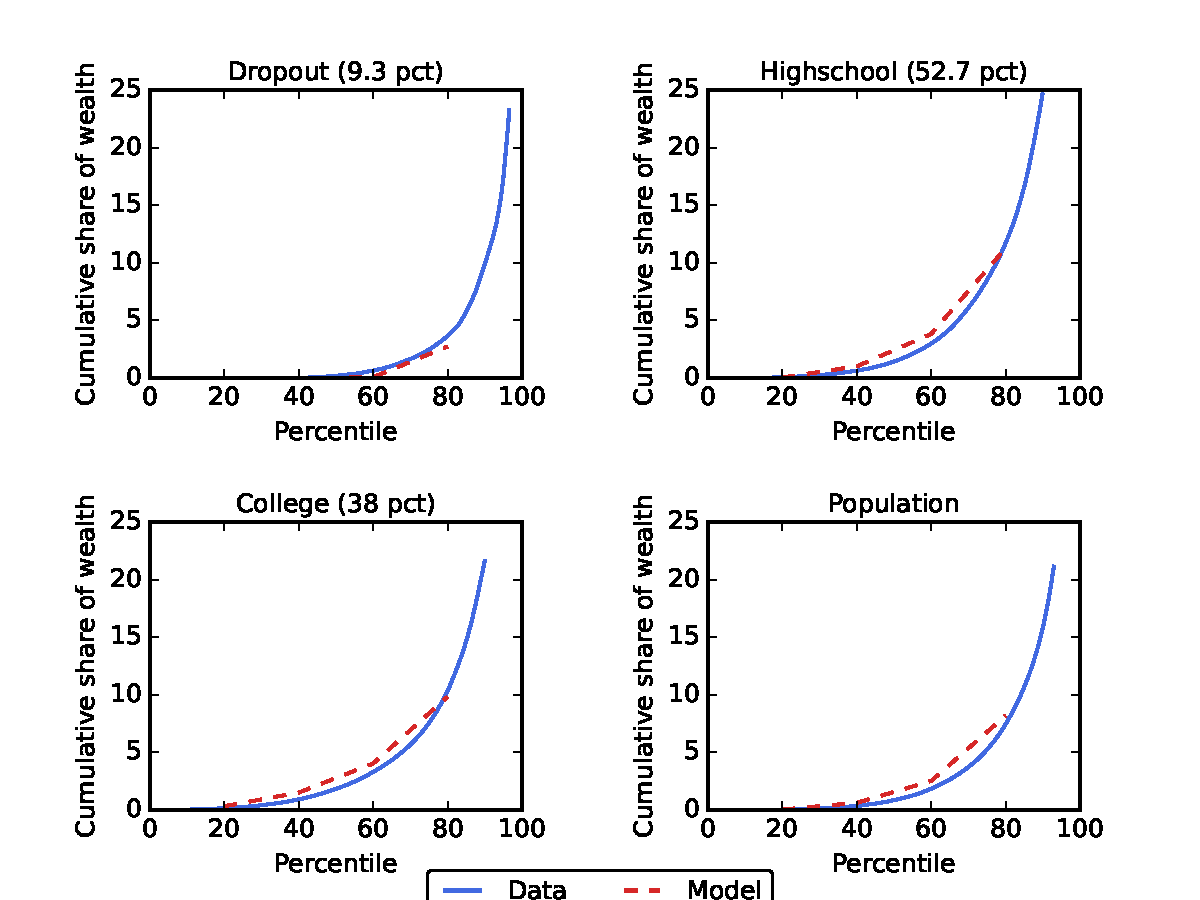
\includegraphics[width=4in]{\FigDir/LorenzPoints.pdf}}
\end{frame}


\section{Results}


\begin{frame}
\frametitle{Impulse responses for stimulus check}

	\begin{figure}
		\centering
		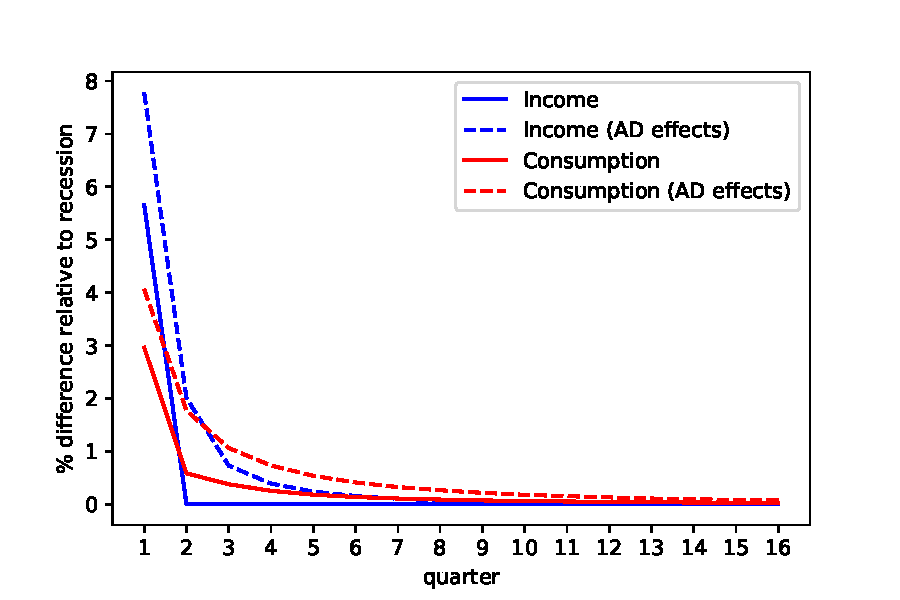
\includegraphics[width=0.6\linewidth]{\econtexRoot/Code/HA-Models/FromPandemicCode/Figures/recession_Check_relrecession}
		\caption{Impulse responses of aggregate income and consumption to a \textbf{stimulus check} during recessions}
	\end{figure}


	\begin{itemize}
		\item Without aggregate demand effects: the first quarter's income is 5.5\% higher; consumption jumps by 3\% 
		\item With aggregate demand effects: first quarter income is 6.5\% higher; consumption elevated for longer time
	\end{itemize}

\end{frame}


\begin{frame}
\frametitle{Impulse responses for extension of unemployment benefits}

	\begin{figure}
		\centering
		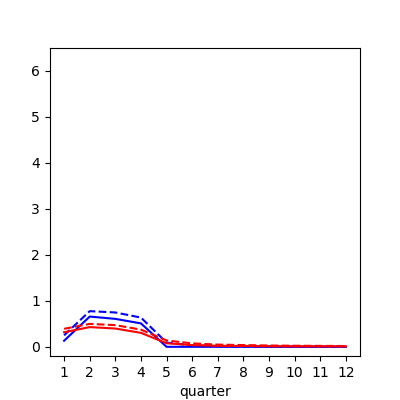
\includegraphics[width=0.6\linewidth]{Code/HA-Models/FromPandemicCode/Figures/recession_UI_relrecession}
		\caption{Impulse responses of aggregate income and consumption to a \textbf{UI extension} (benefit duration increases from 6 to 12 months) during recessions}
	\end{figure}
	
	\begin{itemize}
		\item Without aggregate demand effects: quarterly income increases by max 0.7 percent, consumption response shows anticipation of longer duration
		\item With aggregate demand effects: extra boost to income by 0.2 percent, consumption stays elevated for longer time
	\end{itemize}

\end{frame}


\begin{frame}
\frametitle{Impulse responses for payroll tax cut}

	\begin{figure}
		\centering
		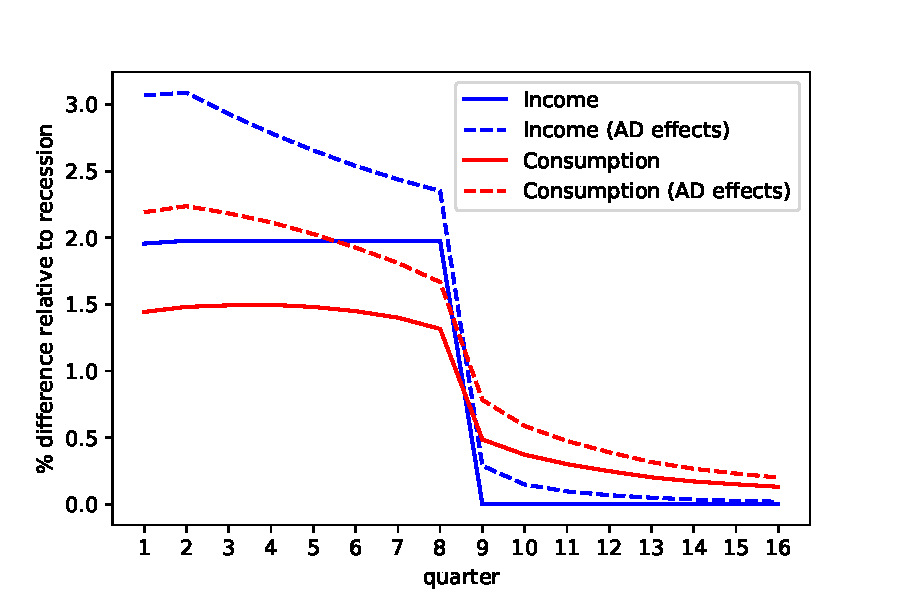
\includegraphics[width=0.6\linewidth]{Code/HA-Models/FromPandemicCode/Figures/recession_taxcut_relrecession}
		\caption{Impulse responses of aggregate income and consumption to a \textbf{payroll tax cut} lasting eight quarters during recessions}
	\end{figure}
	
	
	\begin{itemize}
		\item Without aggregate demand effects: income rises by close to 2 percent; Consumption jumps by 1.5 percent and drops sharply after the income decline.
		\item With aggregate demand effects, income rises by 2.5 percent, declines steadily as the recession's likelihood decreases
	\end{itemize}






\end{frame}




\begin{frame}
\frametitle{Multipliers when aggregate demand effects are present}


\begin{equation*}
M^P_t = \frac{\text{Net present value of policy-induced consumption up to $t$}}{\text{Net present value of the cost of the policy}}
\end{equation*}

\begin{figure}[t]
	\centering
	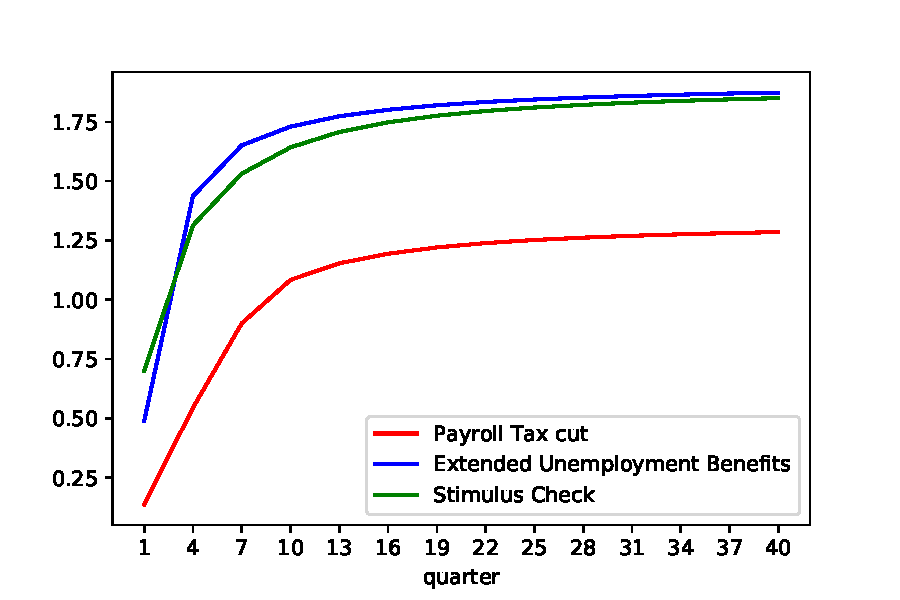
\includegraphics[width=0.6\linewidth]{Code/HA-Models/FromPandemicCode/Figures/Cummulative_multipliers}
	\caption{Cumulative multipliers over time}
\end{figure}

\begin{table}
	\footnotesize
	\begin{tabular}{@{}lccc@{}} 
		& Tax Cut    & UI extension    & Stimulus check    \\ 
		Long-run Multiplier  &1.079  & 1.275  & 1.339     \\ 
		Policy expenditure during recession  &57.6\%  & 80.6\%  & 100.0 \%    \\ 
	\end{tabular}  
\end{table}

\end{frame}

\begin{frame}
\frametitle{Welfare measure construction}

	Guiding principles
	
	\begin{enumerate}
		\item Each consumer is valued equally by the social planner 
		\item Utility from splurge in the same way as other spending
		\item No social benefit to the policies outside of a recession
	\end{enumerate} 
	
	\vspace{0.6cm}
	
	Simple aggregation of consumer util. only satisfies principle 1 \& 2:
	\begin{align*}
	\mathcal{W}(\text{policy},Rec,AD) =\frac{1}{N}\sum_{i=1}^{N} \sum_{t=0}^{\infty} \beta_S^t u(\mathbf{c}_{it,\text{policy},Rec,AD}) 
	\end{align*}
	
	\begin{itemize}
		\item $\mathbf{c}_{it,\text{policy},Rec,AD}$: consumption paths (including splurge) for each consumer / policy
		\item $Rec\in\{1,0\}$: recession indicator, $AD\in\{1,0\}$: AD ind.
		\item $\beta_S = 1/R$: social planner's discount factor 
	\end{itemize}	

\end{frame}


\begin{frame}
\frametitle{Welfare measure construction II}

	To satisfy principle 2 we define $\mathcal{C}(\text{policy},Rec,AD) =$
	\begin{align*}
	& \bigg( \underbrace{\frac{\mathcal{W}(\text{policy},Rec,AD)-\mathcal{W}(\text{None},Rec,AD)}{\mathcal{W}^c}}_\text{\RNum{1}}  - \underbrace{\frac{PV(\text{policy},Rec)}{\mathcal{P}^c} }_\text{\RNum{2}} \bigg) \nonumber \\  
	& -
	\bigg( \underbrace{\frac{\mathcal{W}(\text{policy},0,0) - \mathcal{W}(\text{None},0,0)}{\mathcal{W}^c}}_\text{\RNum{3}}  - \underbrace{\frac{PV(\text{policy},0)}{\mathcal{P}^c}}_\text{\RNum{4}}  \bigg) 
	\end{align*}
	
	\begin{itemize}
		\item \RNum{1}: Policy-induced increase in agg. welfare (in bp of SS-cons.)
		\item \RNum{2}: Cost of policy $\Leftrightarrow$ \RNum{1} - \RNum{2}: Net agg. welfare increase
		\item \RNum{3} - \RNum{4}: Net welfare impact of policy outside of recession
		\item $\mathcal{C}$ measures only welfare effects beyond pure redistribution
	\end{itemize}

\end{frame}


\begin{frame}
\frametitle{Welfare results}

	\begin{table}[ht] 
		\begin{tabular}{@{}lccc@{}} 
\toprule 
                          & Check      & UI    & Tax Cut    \\  \midrule 
$\mathcal{C}(Rec,\text{policy})$ & 0.011  & 0.580  & 0.002     \\ 
$\mathcal{C}(Rec, AD,\text{policy})$ & 0.346  & 1.990  & 0.133     \\ 
\end{tabular}  

	\end{table}

	\begin{itemize}
		\item All policies adjusted to the fiscal size of the UI extension
		\item Interpretation: A welfare gain of x $\Leftrightarrow$ social planner is indifferent between 
		\begin{itemize}
			\item the stimulus policy being implemented in response to a recession and 
			\item a permanent increase in the baseline consumption of the total population by x basis points (0.01\% of baseline cons.)
		\end{itemize}
	
		\item All policies much more effective when mulitplier present
		\item UI extension is clear bang-for-the-buck winner (but limited scalability)
	\end{itemize}


\end{frame}


\begin{frame}
\frametitle{Robustness}
List here all robustness checks performed
\end{frame}


\begin{frame}
\frametitle{Conclusion: Comparing the policies}
Draw conclusions based on results
\end{frame}


\section{Appendix}

\begin{frame}
\frametitle{Appendix I}
\end{frame}


\end{document}

